% !TEX root = ../report.tex

\chapter{Preliminary Study}
% http://www-03.ibm.com/press/us/en/pressrelease/42451.wss

\minitoc

Review of relevant literature;
review of similar software products or tools.

I “survey”-kapittelet presenter en oversikt over tidligere relevant arbeid inkludert artikler og evt. eksisterende produkter.
Vurder kritisk styrker og svakheter av tidligere arbeid



This chapter is ment to outline the preliminary study of our project. This includes
    - what our technologies aims to achieve
    - how we will use them to achieve this.
Beyond this, the chapter will show the mythology the team chose to use and why this was a natural choice to go with. Research in software testing methods will be included and the best fit for this project. Since this is a prototype project, a considerable time is put into this part of the project, to assure the team makes good choices when it comes to technologies to use.

\clearpage

% \section{Set to work with (another name perhaps (or maybe completely removed))}
% About Netflix
\section{Movie Recommendation}
This is the prestudy for the movie recommendation part of the system. We will look at existing recommendations systems, datasets to be explored and how to explore this set.


\subsection{Netflix}
% http://en.wikipedia.org/wiki/Netflix
% http://electronics.howdexstuffworks.com/netflix2.htm
% http://blog.jimjh.com/static/downloads/2013/05/12/netflix.pdf

\begin{wrapfigure}{r}{.30\textwidth}
\vspace{-30pt}
\centering

\includegraphics[width = .25\textwidth]{image/netflix-logo.png}
\end{wrapfigure}

Netflix is a on-demand Internet streaming media. It started out as a DVD-rental business, but moved over to a more Internet based business model in 1999 and have from then on had a great success in the subscription-based digital distribution service. To improve customer satisfaction they developed a personalized video-recommendation system called Cinematch. About 60\% of the Neflix users select their next movie or TV-show based on this recommendation[------------------2---------------], so it is important that this recommendation system manages to capture the users movie and TV-show preferences and feed back fitting movies and TV-shows.

\subsubsection{Cinematch}
\label{subsec:Cinematch}
% http://electronics.howstuffworks.com/netflix2.htm
This recommendation system is self-updating. It searches the Cinematch database for users who have rated the same movie, determents which of these again have rated a second movie and with this calculates likelihood that users who like the first also likes the second one.


\subsection{The Dataset}\label{subsec:netflixdata}
% Pages used:
% http://www.timelydevelopment.com/demos/NetflixPrize.aspx
% http://dl.acm.org/citation.cfm?id=1536622&jmp=cit&coll=portal&dl=ACM#CIT
% http://www.the-ensemble.com/content/netflix-prize-movie-similarity-visualization
% http://en.wikipedia.org/wiki/Netflix_Prize
% http://blog.jimjh.com/static/downloads/2013/05/12/netflix.pdf
% http://en.wikipedia.org/wiki/Root-mean-square_deviation

Netflix held a competition where the contest was made to help Netflix improve their movie recommendation system. The team that could beat Netflix's own collaborative filtering system by more than 10\% could win one million dollars. To measure the score root-mean-square error (RMSE) was used, which is used to measure the difference between the values predicted or estimated and the actual values observed. The RMSE of Cinematch~\ref{subsec:Cinematch} was at 0,9525.

\subsubsection{Root-mean-square error RMSE}

\begin{equation}\label{eq:rmse}
RMSE = \sqrt {{\frac{{\sum\limits_{{i = 1}}^n {{{\left( {{y_i} - {{\hat{y}}_i}} \right)}^2}} }}{{n}}}}
\end{equation}

The equation for calculating the RMSE is show in figure~\ref{eq:rmse}. It calculates how far the estimated value is from the actual value. Here ${y_i}$ is the actual value and ${\hat{y}}$ is the estimated value. The square difference of all the values are averaged, where ${n}$ is the number of values, this result is rooted. This produces the average distance of all the values the estimate is from the actual.


\subsubsection{Competition}

For this competition Netflix produced a training dataset based on user ratings from their own database. It contains 100 480 507 ratings from 480 189 unique users on 17 770 movies. The data is split up into 17 770 files, one for each movie, where the data is a triplet of the form <user, rating, date-of-rating>. The user-field and rating-field is an integer, while the date-of-rating-field is on the ISO 8601 form, year-month-day. The different movies have different amounts of ratings, and the different users have rated different amounts of movies.

With the training dataset the teams system was supposed to predict ratings on a "qualifying"-dataset, which contained 2 817 131 triplets with only user ids, movie ids and dates. This "qualifying"-datase must be disregarded since the actual ratings for this dataset was only know to the jury of the competition and is nowhere to be found. Instead a probe set is provided with 1 408 385 users which can be used to remove these from the training set to test predictions based on the test set. This probe set possesses similar statistical values as the qualifying set, so it will give a good prediction of how the result actually would have scored in the competition.

\begin{center}
\begin{tabularx}{\textwidth}{ l X }
\hline
\textbf{Ratings} & 100 480 507 \\ \hline
\textbf{Customers} & 480 189 \\ \hline
\textbf{Movies} & 17 770 \\ \hline
\textbf{Qualifying set} & 2 817 131 \\ \hline
\textbf{Probe set} & 1 408 385 \\ \hline
\end{tabularx}
\captionof{table}{Dataset statistics}\label{tab:nfDatasetStat}
\end{center}


\subsubsection{Dataset statistics}
% http://en.wikipedia.org/wiki/Principal_components_analysis
% http://en.wikipedia.org/wiki/Singular_value_decomposition
% http://en.wikipedia.org/wiki/Latent_semantic_indexing
% http://www.timelydevelopment.com/demos/NetflixPrize.aspx

To better understand the dataset, some statistics about the dataset was produced.

\begin{figure}[H]
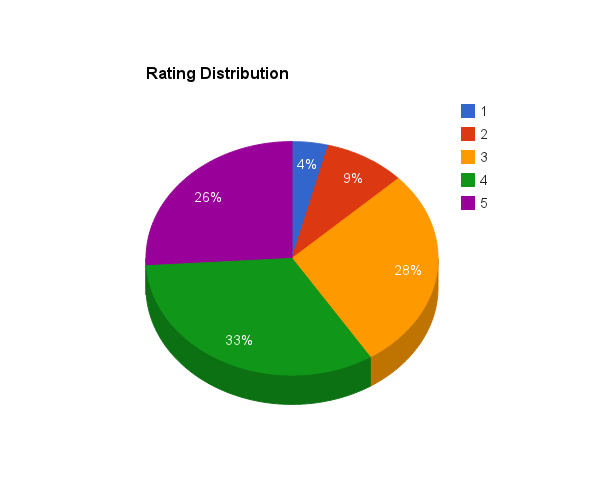
\includegraphics[width=5in]{image/ratingdistr.png}
\centering
\caption{Rating distribution}
\label{figure:ratingdistr}
\end{figure}

Rating distribution is shown in figure~\ref{figure:ratingdistr}. 1/3 of the ratings are 4, and rating 1 and 2 only makes up for 13\% of the rating distribution. 3 and 5 are quite similarly represented with 28\% and 26\% respectively. It can from this be assumed a greater prediction towards the higher ratings, and predictions towards lower ratings should not be done lightly.

\begin{figure}[H]
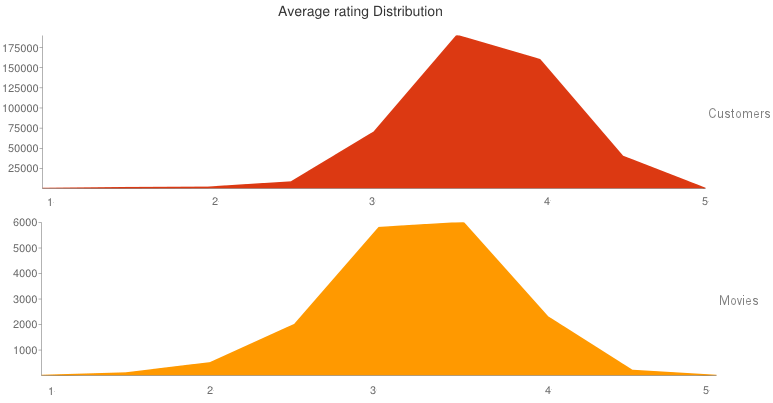
\includegraphics[width=5in]{image/avgratingdistr.png}
\centering
\caption{Average rating distribution}
\label{figure:avgratingdistr}
\end{figure}

\begin{figure}[H]
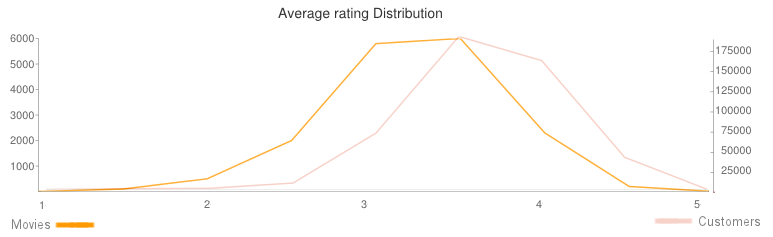
\includegraphics[width=5in]{image/avgratdistrover.png}
\centering
\caption{Average rating distribution}
\label{figure:avgratdistrover}
\end{figure}


Average rating distribution is shown in figure~\ref{figure:avgratingdistr}. The upper graph shows average rating distribution of the customers, while the bottom one shows the distribution per movie. Both graphs have quite similar form. Both customers and movies peak at a rating of 3,5, which is natural. The second second highest point is for the customers at 4 and movies at 3, which is interesting to see. TO ANALYSE MORE!


\begin{figure}[H]
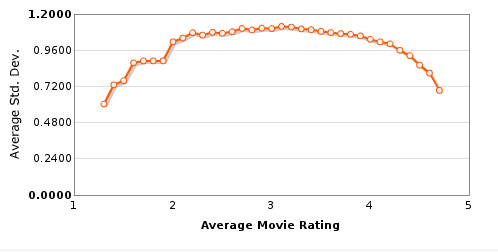
\includegraphics[width=5in]{image/avgmovierating.png}
\centering
\caption{Average movie rating distribution}
\label{figure:avgmovierating}
\end{figure}

Average movie rating distribution is shown in figure~\ref{figure:avgmovierating}. Here we see that for the edge ratings (rating 1 or 5) has the least standard deviation, so when a movie is highly rated it usually is rated high, and the same goes for low ratings, while for the middle ratings (2 to 4) we see that it variates more, and quite similarly. So the middle ratings are harder to classify, in other words, when a movie has a rating of 3, the average rating-shift is almost 1.1, so it must be expected that there is a bigger classification hit on these, so the problem will be to fin the right classification.




\subsection{What the top Netflix-Prize contestants did}\label{subsec:thewinners}

\subsubsection{BellKor's Pragmatic Chaos}
% http://www.stat.osu.edu/~dmsl/GrandPrize2009_BPC_BellKor.pdf
% http://www2.research.att.com/~volinsky/netflix/
% http://www.netflixprize.com/assets/GrandPrize2009_BPC_PragmaticTheory.pdf
% http://www.netflixprize.com/assets/GrandPrize2009_BPC_BigChaos.pdf
% http://blog.revolutionanalytics.com/2009/09/bellkor-wins-netflix-prize.html
% http://www.wired.com/business/2009/09/how-the-netflix-prize-was-won/
% http://www.netflixprize.com//community/viewtopic.php?id=1537

BellKor's Pragmatic Chaos, the prize winners of the Netflix-Prize competition, was a group of scientists from AT\&T Labs, Yahoo!, Pragmatic Theory and Commendo Research \& Consulting. They achieved a RMSE of 0.8567, which was 10.06\% better than Netflix's own Cinematch score.

Models for the rating data is learned by fitting previously observed ratings, but since the model is to be used to predict feature ratings, overfitting the data. This achieved by regularizing the learned parameters. A regularization constant is used, and is set to L2 by default. This and other constant such as, step size and number of iterations are set manually through greedy manners. Where the algorithm is ran multiple times and constant value with best score is used. \cite{BellKor-PragmaticTheory}

The winning algorithm was put together based on multiple different modeling techniques. Some of these modeling techniques are described in table~\ref{table:bellkor-models}

\begin{table}[H]
\caption{Some of the models the "The BellKor's Pragmatic Chaos"-team used \cite{BellKor-PragmaticTheory}}
\centering
\begin{tabular}{ p{3.2cm} p{9cm} }
\hline
  \textbf{Model} & \textbf{Description}\\
  \hline \\ [-1.5ex]
  Time of week rating & The team saw that a user-rating done in the weekends had a tendency to have a higher value than a rating done on a Monday. This also applies for multiple ratings done the same day, higher ratings does not necessarily imply that the movie is much better than a movie rated lower another day, the user might just be in a good mood. \\
  \hline \\ [-1.5ex]
  Close User ratings & Ratings done close to one another done by the same user implied that the user was rating based on the user's recollection of the rated movies, and not that the user just saw that movie, these ratings had to be handled in its own manner. This was because of the effect the faulty or old memories had on these ratings. The all time favorites/negatives are also usually in this bulk. While the movies which did not make much of an impression are forgotten. This helps us explain \ref{figure:avgmovierating}, where we saw that movies with the edge ratings (1 or 5) had a lower rating distribution. \\
  \hline \\ [-1.5ex]
  Baseline predictors & Some users has the tendency to rate on an overall average higher than other users.\\
  \hline \\ [-1.5ex]
  Movie like-ability & Movies can go in and out of popularity. This change usually happens over a extended period. \\
  \hline \\ [-1.5ex]
  Frequency term & The number of ratings a users gives on a specific day can help explains data-variability during that day. \\
  \hline \\ [-1.5ex]
  Matrix factorization with Temporal Dynamics & Use two sets pf static movie factors. Set one is used in all the models of the factors. Set two uses the movies rated by the user, normalizes the sum, and uses this as a user factor. \\
  \hline \\ [-1.5ex]
  Neighborhood model with Temporal Dynamics & Most common approach to collaborative filtering. They used a item-item model based on global optimization. To predict rating of a new item based of rating an old item two sets of weights where used. One where the values of the ratings where accounted for, and one disregarding rating values.
  A situation where a user rates an old item and a new item close to each other both in time and rating, is a better indicator that these items can be related to each other, than if two items are rated similarly, but with a greater timespan between each other.Therefore a decaying relationship is introduced between items. This decreased RMSE from 0.9002 to 0.8870.\cite{BellKor-CF-TD} \\
\end{tabular}
\label{table:bellkor-models}
\end{table}

Interestingly, the bias model with tanking in the factor that users change rating-scale over time, resulted in a RMSE of 0.9555, which is almost as good as the Cinematch Netflix was already using. The learning with the different modeling techniques is done by a stochastic gradient descent algorithm running for 30 iterations. This is the only time they use an automatic parameter tuner. \cite{BellKor-2008-sol}

As we can see from table~\ref{table:bellkor-models} the "BellKor's Pragmatic Chaos"-team used a lot of different models and did a lot of tweaking to get to the top. Some interesting findings to take from this is the importance of diversity and how central the timestamp of a rating can be.

\subsubsection{The Ensemble}
% http://www.the-ensemble.com/

A merger of the teams "Grand Prize Team" and "Opera Solutions and Vandelay United". They also managed to get a RMSE of 0.8567, and therefore a 10.09\% improvement as well. But lost since the "BellKor's Pragmatic Chaos"-team managed to submit their results 20 minutes earlier than "The Ensemble"-team.

The two merged teams, which made "The Ensemble" consisted of multiple smaller teams. They had all competed in the Netflix-Prize challenge, and had to put their heads and code together to get to the result they got to.

"The Ensemble"-team used a huge variation of models, just as the "BellKor's Pragmatic Chaos"-team.

After the competition was done "The Ensemble" tested a merger of their system with the "BellKor's Pragmatic Chaos"-system. The test RMSE of a 50/50 blend was 0.855476, which is a 10.19\% improvement. This is 0.10\% better then the teams managed to produce by themselves.

\subsubsection{Conclusion}
After looking at the two top contestants from the competition a pattern is starting to form. Diversity is key to be able to predict user-ratings at a top level.

% End Netflix



% About Weka
\section{Weka}
%http://en.wikipedia.org/wiki/Weka_(machine_learning)

\begin{wrapfigure}{r}{.30\textwidth}
\vspace{-30pt}
\centering

\includegraphics[width = .25\textwidth]{image/Weka-logo.png}
\end{wrapfigure}


Weka is a machine learning software written in Java. It can be used to visualize data through analyzing it with different kinds of algorithms. The Explorer, a graphical user interface, makes it easy to work with and explore data from different angles. It is a free software under the General Public License \cite{GNU}. Weka can handle several data mining tasks, including, data preprocessing, clustering, classification, regression and feature selection. The input data has to be a single flat file or relation, each data point must be described by a fixes number of attributes. The dataset can be accessed trough a SQL database. Can link database tables into a single datatable, which can be used for processing using Weka.


\subsection{ARFF}
% http://www.cs.waikato.ac.nz/ml/weka/arff.html
Attribute Relationship File Format is the file type used to store data in a database. The structure is as follows:

\begin{lstlisting}[caption={ARFF Example},label={lst:arffEx},captionpos=b]
@relation 'flat-netflix'

@attribute assetId string
@attribute 14367 numeric
@attribute 6050 numeric
@attribute 14112 numeric

@data
1658496,?,?,4
684232,3,3,?
684231,4,?,?
1774519,1,?,?
\end{lstlisting}

Listing~\ref{lst:arffEx} is an example of how an ARFF file is structured. It startes with a header, containing "@relation", "@attribute"s and the "@data". This header defines the name of the relation, the attributes in the dataset and the data. The "@data"-header contains arrays, where each array has values for the corresponding "@attribute"s values. If a array has no value for a particular attribute it is denoted as a question mark (?).

\subsection{The Explorer}
% http://www.cs.waikato.ac.nz/~ml/weka/gui_explorer.html
% http://research.cs.queensu.ca/home/cisc333/tutorial/Weka.html
% http://wiki.pentaho.com/display/DATAMINING/Time+Series+Analysis+and+Forecasting+with+Weka
\begin{table}[H]
\centering
\begin{tabularx}{1.0\textwidth}{ l p{9.3cm} }
  \textbf{Components} & \textbf{Description} \\
  \hline \\ [-1.5ex]
  Preprocess & Here the user can import the data which is going to be analyzed. It is also possible to do some filtering on this data, this includes removing of values and transforming values. \\
  \hline \\ [-1.5ex]
  Classify & Here the user can apply classification and regression algorithms to the dataset. \\
  \hline \\ [-1.5ex]
  Associate & Here the user can have the association rule learners identify important relationships between attributes in the provided dataset. \\
  \hline \\ [-1.5ex]
  Cluster & Here the user can apply cluster algorithms to the dataset \\
  \hline \\ [-1.5ex]
  Select attributes & Here the user can identify the most predictive attributes in the dataset. \\
  \hline \\ [-1.5ex]
  Visualize & Here the user can get a visualization of the dataset, and of the different algorithms preformed on the dataset. \\
\end{tabularx}
\caption{Classification based on feature}
\label{table:nosql-calssifications}
\end{table}


\subsection{Using Weka to analyze the netflix-data}


% End Weka




% About Twitter
\section{Twitter}\label{sec:twitter}

\begin{wrapfigure}{r}{.30\textwidth}
\vspace{-30pt}
\centering

\includegraphics[width = .25\textwidth]{image/twitter-logo.png}
\end{wrapfigure}
Twitter is a free social media network based on microblogging. In microblogging, a user can post a paragraph of a certain number of characters or less to his/her timeline. The user can also follow other users. Whenever the users that a given user is following posts something, the user can see these posts in his/her feed. This is the basis for many of todays most popular social media networks, including Twitter.

\subsection{Terminology}
For more clarity, we define the terminology twitter uses. All words in \textbf{bold} are our own definitions for more easily describing how the various term relate to eachother.

\subsubsection{Tweet}
A tweet is a post containing max 140 characters. It can also refer to the verb ‘to tweet’, which means ‘to post a tweet’. \textbf{tweets} is an attribute of a user which returns a list of tweets that the users

  \textbf{user.tweets -> [<tweet>]}
\subsubsection{User}
A user is someone with a twitter account. A user can post tweets. By following other users, twitter generates a feed for the user containing the tweets of all the users they follow. They also have certain information retrieval tools available, such as filtering tweets by a tag name, specific user or search term.

\subsubsection{Tweeter}
A user who tweets a tweet that is referenced in the same context. For instance: The best tweets are tweeted by the most popular tweeters


\subsubsection{Follower}
A follower is someone who follows a user. The follower will see the users tweets in their feed. \textbf{followers} is an attribute of a user which returns the list of users that are following that user.

  \textbf{user.followers -> [<user>]}

\subsubsection{Followee}
A followee is someone who a user is following. The user will appear in the followees list of followers, and the followee will appear in the users list called ‘following’. We will refer to the list ‘following’ for a user as followees for clearer terminology. \textbf{followees} is an attribute of a user which returns the list of users that the user is following.

  \textbf{user.followees -> [<user>]}

\subsubsection{Hashtag}
Hashtags are topic labels that are placed on tweets. They are made by typing \#topicname anywhere in the tweet. By navigating to \#topicname, a user will see a feed of all tweets containing \#tagname. \textbf{hashtags} is a an attribute of a tweet which returns the list of hashtags the tweet contains.

  \textbf{tweet.hashtags -> [<hashtag>]}

\noindent
Hashtag also has the attribute tweets, which returns all tweets that have a certain hashtag. These hashtags are ordered by twitters algorithm which balances how recent the tweet is with the popularity of the tweeter.

  \textbf{hashtag.tweets -> [<tweet>]}

\subsubsection{Usertag}
Usertags are labels that are placed on tweets describing who the tweets are adressed to. They are made by typing @username anywhere in the tweet. This tweet will also show up in the feed of the user with name username. \textbf{usertags} is an attribute of a tweet which returns the list of users that the tweet is adressed to.

\textbf{tweet.usertags -> [<user>]}

\subsection{REST API}
Twitters HTTP/HTTPS based REST API allows the application using it to perform many of the core functionalities of Twitter. The fully reflects Twitter's content.

\subsubsection{Usage}
The API is divided into POST and GET requests. The POST requests makes changes to twitter. A POST request could be for posting a tweet, update a users profile etc. The GET requests retrieves data from twitter. A GET request could be used to retrieve followees or followers of a user, retrieve the tweets on the timeline of a user etc. The data is returned as JSON. \cite{twitter-rest-api}

\subsubsection{Authentication}
Twitters REST API uses an access token generated for the specific application in order to make a request. In addition, OAuth can be used if the session is on behalf of a specific user. Some requests such as posting a tweet can of course only be made on behalf of a user and thus requires OAuth. \cite{twitter-rest-api}

\subsubsection{Rate Limit}
The number of requests an application or a user can make is limited to a 15 minute window. Within this 15 minute window the each user can make 15 GET requests. This means that a user can retrieve the followees of 15 users withing the 15 minute window, but must wait until the 15 minutes have passed before retrieving more data. This means that large amounts of data can only be retrieved over long periods of time.

If only the application access token is used and not OAuth, the application as a whole can make 15 GET requests within the window. \cite{twitter-rate-limiting}

\subsection{Search API}
Twitters Search API is a REST API that is used for searching for tweets that match a search query.

\subsubsection{Usage}
The Search API uses only GET requests. Each GET request contains the search query as well as other parameters such as location to specify the search further. The API will return tweets that contain any of the words in the search query in any order. The tweets are returned as JSON.\cite{twitter-rest-api}

It is important to note that not all tweets are indexed in the Search API. Only a selected number of tweets, possibly within only a certain time frame are available. The tweets returned by the Search API are thus only a subset of all tweets.\cite{twitter-search-api-timeframe}

\subsubsection{Authentication}
To authenticate, the access token generated for the application can be used as well as OAuth. This is the same as the REST API. \cite{twitter-rest-api}

\subsubsection{Rate Limit}
The number of requests that can be made are limited to 180 requests per 15 minute window for each OAuth. If the Search API is accessed using only the application access token, these limitations apply application-wide for any number of users.\cite{twitter-rate-limiting}

\subsection{Stream API}
\subsubsection{Authentication}

\subsection{Crawling and Scraping Twitter}
TODO: Add appendixes from scrapbook.
This section will examine how to crawl Twitter using Twitters HTTPS Web Search. This will be examined by browsing twitter.com logged in as a user and examining it Google Chrome Developer Tools (GCDT)\cite{gcdt} as the site is being browsed and search requests are being made. The goal of this examination is to discover requests a webcrawler must be capable of making in order to search twitter and harvest tweets and users automatically.


\subsubsection{Search Request}
TODO: Labels for all snippets in this section.
Tweets can be found using an HTTPS search request with the search query in the format URLE [1]
TODO: URLE Reference.
Searching for <URLE search query> can be done with the following request.
TODO: Make <URLE-search-query> clearer in url

  \url{https://twitter.com/search?q=<URLE-search-query>&src=typd&f=realtime}

In the rest of the discussion of search, we'll be using the following query as an example. This is a search request for the search query "The Dark Knight Rises 2012".

  \url{https://twitter.com/search?q=the%20dark%20knight%202012&src=typd&f=realtime}

Using the Google Chrome Developer Console [2] we can find the DOM elements on the search page that contain the tweets that have been returned, using the select element tool. We'll refer to this as the tweets element.

  \begin{lstlisting}[caption={Tweet Element},label={},captionpos=b]
  <ol class="stream-items js-navigable-stream" id="stream-items-id\">
  \end{lstlisting}

The first element contained within the tweets element is a summary of the users who have posted the tweets returned by the search, and is not of interest.

The rest of the li-elements in the tweets element contain tweets elements. They have the following format

  \begin{lstlisting}[caption={Tweet Element},label={},captionpos=b]
  <li class="js-stream-item stream-item stream-item expanding-stream-item" data-item-id="397530125715402752" id="stream-item-tweet-397530125715402752" data-item-type="tweet">...</li>
  \end{lstlisting}

TODO: Create reference for jQuery
Using jQuery [3] and the Javascript Console in GCDT \cite{gcdt}, we can determine how many tweets have been returned. To do this, we define a javascript function that selects the tweets element dom element, gets a list of it's children and counts the number of items in this list and subtract 1 for the user summary element.

  \begin{lstlisting}[caption={TODO: Caption},label={},captionpos=b]
  > number_of_tweets_in_search_results = function(){ return $("li[data-item-type='tweet']").size(); }
  > number_of_tweets_in_search_results();
  15
  \end{lstlisting}

\subsubsection{Scroll Search Results}
In order to obtain more search results it is necessary to scroll to the bottom of the page for the browser to make an XHR request to retrieve more tweets. As the scrolling is done, XHR requests can be monitored in the Network tab of GCDT. Consecutive xhr requests are sent as scrolling is done several times.

  \begin{lstlisting}[caption={TODO: Caption},label={},captionpos=b]
  Javascript Console:
  > number_of_tweets_in_search_results();
  15

  Network Console > XHR:
  Request URL:https://twitter.com/i/search/timeline?q=the%20dark%20knight%202012&src=typd&include_available_features=1&include_entities=1&last_note_ts=0&scroll_cursor=TWEET-360758159364734978-399762568459612160


  Javascript Console:
  > number_of_tweets_in_search_results();
  35

  Network Console > XHR:
  Request URL:https://twitter.com/i/search/timeline?q=the%20dark%20knight%202012&src=typd&include_available_features=1&include_entities=1&last_note_ts=0&oldest_unread_id=0&scroll_cursor=TWEET-338938038694584320-399762568459612160

  Javascript Console:
  > number_of_tweets_in_search_results();
  50

  Network Console > XHR:
  Request URL:https://twitter.com/i/search/timeline?q=the%20dark%20knight%202012&src=typd&include_available_features=1&include_entities=1&last_note_ts=0&oldest_unread_id=0&scroll_cursor=TWEET-316893896573607937-399762568459612160

  Javascript Console:
  > number_of_tweets_in_search_results();
  65
  \end{lstlisting}

As the requests are sent and processed, tweets are appended to the tweets element. All that is needed in order to keep receiving tweets is to keep sending requests of this pattern.
Examining the requests attributes, they consists of the following variables and constants.

  \begin{lstlisting}[caption={TODO: Caption},label={},captionpos=b]
  constant src=typd
  constant include_available_features=1
  constant include_entities=1
  constant last_note_ts=0
  constant oldest_unread_id=0
  variable scroll_cursor=TWEET-<18 character number>-<18 character number>
  \end{lstlisting}

At this point a snapshot of the html page is taken [A3]. The only attribute that seems to variate with each request is scroll\_cursor attribute. This means that the piece of javascript code that is making the requests somehow has access to the information contained in this changing attribute. A quick dom tree search for 'TWEET-' shows us that scroll\_cursor is contained by a div with the class stream-container under under the attribute 'data-scroll-cursor' and 'data-refresh-cursor'.

  \begin{lstlisting}[caption={TODO: Caption},label={},captionpos=b]
  <div class="stream-container" data-scroll-cursor="TWEET-311337362556846081-399762568459612160" data-refresh-cursor="TWEET-396773826303762432-399762568459612160">
  \end{lstlisting}

By making another scroll to the bottom of the page, a request with scroll-cursor information from one of these attributes is sent.
As is shown, the attribute data-scroll-cursor is responsible for what goes in the attribute scroll-cursor.

  \begin{lstlisting}[caption={TODO: Caption},label={},captionpos=b]
  Network Console > XHR:
  https://twitter.com/i/search/timeline?q=the%20dark%20knight%202012&src=typd&include_available_features=1&include_entities=1&last_note_ts=0&scroll_cursor=TWEET-311337362556846081-399762568459612160
  \end{lstlisting}

\subsection{Scraping Search Results}

Each tweet element in the search results contains DOM elements of importance that can be scraped. These DOM elements are shown in table-\ref{table:important-tweet-element-elements}.

\begin{table}[H]
\centering
\begin{tabularx}{5.3\textwidth}{ lp{7cm} lp{5cm} }
  \textbf{Element Name} & \textbf{Content}\\
  \cline{0-1}
  User ID & The ID of the user who posted the tweet \\
  \cline{0-1}
  User Name & The name of the user who posted the tweet \\
  \cline{0-1}
  Text & the text contained in the tweet
\end{tabularx}
\caption{Elements to be scraped from each tweet element that have been retrieved}
\label{table:important-tweet-element-elements}
\end{table}

\subsubsection{User}
The user name can be found in the header of the tweet. Using the GCDT Select, it can be extracted from the page. It will be referred to as the user name element.

\begin{figure}[H]
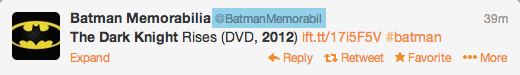
\includegraphics[width=4in]{image/tweet-user-field.png}
\centering
\caption{User name element (shown in blue) in a tweet retrieved by twitter web search}
\label{figure:tweet-user-field}
\end{figure}

\begin{lstlisting}[caption={HTML of the user name element in a tweet},label={user-name-element-html},captionpos=b]
  <span class=\"username js-action-profile-name\"><s>@</s><b>BatmanMemorabil</b></span>
\end{lstlisting}

\noindent
Using jQuery, a function can be created to count the occurances of the class "username js-action-profile-name".

\begin{lstlisting}[caption={Creating a function in GCDT Javascript Console for counting the occurance of user name elements on the twitter search result page},label={user-name-element-count-jquery-function},captionpos=b]
  > number_of_tweet_user_name_element_occurances = function(){ return $("span.username.js-action-profile-name").size() }
\end{lstlisting}

\noindent
In listing-\ref{user-elements-matches-tweets}, the number of user name elements in the dom tree is compared to the number of tweets in the search result. Since they are equal, it is likely that the right class is being scraped for the user name element.

\begin{lstlisting}[caption={Running functions in GCDT Javascript Console to show that the number of user name elements matches the number of tweets},label={user-elements-matches-tweets},captionpos=b]
  > number_of_tweet_user_name_element_occurances();
  119
  > number_of_tweets_in_search_results();
  119
\end{lstlisting}

\noindent
The user ID can also be found in the header. The ID is contained in the attribute data-user-id. Using the GCDT Select, it can be extracted from the page. It will be referred to as the user id element.

\begin{lstlisting}[caption={TODO: Caption and label},label={},captionpos=b]
  <a class="account-group js-account-group js-action-profile js-user-profile-link js-nav" href="/username" data-user-id="userid">...</a>
\end{lstlisting}

Using jQuery, a function can be created to count the occurances of the class "account-group js-account-group js-action-profile js-user-profile-link js-nav".

\begin{lstlisting}[caption={TODO: Caption and label},label={},captionpos=b]
  > number_of_tweet_user_id_element_occurances = function(){ return $("a.account-group.js-account-group.js-action-profile.js-user-profile-link.js-nav").size() }
\end{lstlisting}

Correlating this with the number of tweets in the search result, shows that this is the right class to crawl for.

\begin{lstlisting}[caption={TODO: Caption and label},label={},captionpos=b]
  > number_of_tweet_user_id_element_occurances();
  21
  > number_of_tweets_in_search_results();
  21
\end{lstlisting}

Content
....
The text can be found in the center of the tweet in the same container as the URL. GCDT Select extracts it from the page. It will be referred to ass the tweet content element.

  \begin{figure}[H]
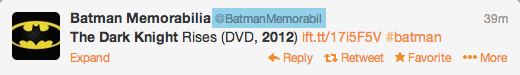
\includegraphics[width=4in]{image/tweet-user-field.png}
\centering
\caption{Text, URL and hastag field (shown in blue) in a tweet retrieved by twitter web search}
\label{figure:tweet-user-field}
\end{figure}

\noindent
This gives us the following dom element.

\begin{lstlisting}[caption={TODO: Caption and label},label={},captionpos=b]
  <p class="js-tweet-text tweet-text">
    <strong>The Dark Knight</strong> Rises (DVD, <strong>2012</strong>)
    <a href="http://t.co/p8pr9wqC4k" rel="nofollow" dir="ltr" data-expanded-url="http://ift.tt/17i5F5V" class="twitter-timeline-link" target="_blank" title="http://ift.tt/17i5F5V">
      <span class="tco-ellipsis"></span>
      <span class="invisible">http://</span>
      <span class="js-display-url">ift.tt/17i5F5V</span>
      <span class="invisible"></span>
      <span class="tco-ellipsis">
        <span class="invisible">&nbsp;</span>
      </span>
    </a>
    <a href="/search?q=%23batman&amp;src=hash" data-query-source="hashtag_click" class="twitter-hashtag pretty-link js-nav" dir="ltr">
      <s>#</s><b>batman</b>
    </a>
  </p>
\end{lstlisting}

Using jQuery, a function can be created to count the occurances of the class "js-tweet-text tweet-text".

\begin{lstlisting}[caption={TODO: Caption and label},label={},captionpos=b]
  > number_of_tweet_content_element_occurances = function(){ return $("p.js-tweet-text.tweet-text").size() }
\end{lstlisting}

Correlating this with the number of tweets in the search result, shows that this is the right class to crawl for.

\begin{lstlisting}[caption={TODO: Caption and label},label={},captionpos=b]
  > number_of_tweet_content_element_occurances();
  119
  > number_of_tweets_in_search_results();
  119
\end{lstlisting}

Text
....
Everything in paragraphs with the class "js-tweet-text tweet-text" that is not a link, is the tweet text.

\begin{lstlisting}[caption={TODO: Caption and label},label={},captionpos=b]
  <strong>The Dark Knight</strong> Rises (DVD, <strong>2012</strong>)
\end{lstlisting}

\subsection{Datamining Twitter for Recommendations}
% End Twitter




\section{Similar solutions (Evaluation of State-of-the-art)}
% http://movielens.umn.edu/login
% http://www.grouplens.org/datasets/movielens/

In this section, we will discuss similar solutions and their relevance to our project.

If this is not state of the art stuff, maybe separate this and that


\subsection{MovieLens}\label{subsec:MovieLens}
Need to rate 20 movies

\subsection{MovieTweetings}
MovieTweetings is an application for fetching movie ratings through the Twitter API from Twitter. The application search for ratings forwarded from IMDB, a movie information webpage, and stored in an accessible

use the social media to get a fresher dataset than using Netflix dataset, or MovieLens datasets~\ref{subsec:MovieLens}. At the time of writing the article they had more than 60 000 ratings, and about 500 new where added every day\cite{MovieTweetings}. They get these ratings from Twitter~\ref{sec:twitter}. The ratings fetched from Twitter are actually ratings from a movie rating and information page, IMDB, which are forwarded to the raters Twitter account. The Twitter API is queried daily to update their database.

While querying the API for well structured tweets with ratings about movies are a good way to go when in search for a database with movie ratings, the data will be sparse. The data is not based on the users followers/followees, and will therefore not represent the social strength Twitter is capable of producing. A direct access to IMDB, rather than going through Twitter to get the rating information also seems like a simpler and more result-producing idea.


\subsection{Twittomender}
\cite{twittomender}







\section{Collaborative Filtering}
% About Classification
% http://www.netflixprize.com/assets/GrandPrize2009_BPC_PragmaticTheory.pdf
% http://www.netflixprize.com/assets/GrandPrize2009_BPC_BellKor.pdf
% http://www.netflixprize.com/assets/GrandPrize2009_BPC_BigChaos.pdf
% http://www2.research.att.com/~volinsky/netflix/Bellkor2008.pdf
% http://public.research.att.com/~volinsky/netflix/cfworkshop.pdf
% http://public.research.att.com/~volinsky/netflix/BellKorICDM07.pdf
% http://www2.research.att.com/~volinsky/netflix/ProgressPrize2007BellKorSolution.pdf
% http://public.research.att.com/~volinsky/netflix/sigkddexp.pdf
% http://www.netflixprize.com//leaderboard
% https://sites.google.com/site/xlvector/netflixprize/papers
% http://www.slideshare.net/bmabey/svd-and-the-netflix-dataset-presentation
% http://lenskit.grouplens.org/

% https://github.com/cloudera/oryx

How to best make something out of the dataset
How to produce the RMSE
What is the RMSE


TODO:
There are two basic problems when analysing very large datasets:
    - Writing the code correctly.
    - The performance (i.e. speed at which it runs).



Something about why and which classification alg to use
% http://scenic.princeton.edu/network20q/wiki/index.php?title=Q4:_How_does_Netflix_recommend_movies%3F
% http://blog.jimjh.com/static/downloads/2013/05/12/netflix.pdf
There were 51 051 contestants on 41 305 different teams competing in the Netflix-Prize competition, and a lot of these contestants shared their solution through code repositories such as GitHub (--------------something about github here?--------------). Since many of these solution scored very well on the contest it was natural to explore these and use their solution to test potential improvement in collaboration with the social media data harvested from Twitter.

Here we explore some of the better solutions and how and why these could be used to our benefit.
Here we explore some of the better solutions and put together how these can be used to


The moivie-suggestion algorithm:


\subsection{Using the Netflix-data}
The Netflix-data has, as mentioned in the section about the dataset \ref{subsec:netflixdata}, a set of ratings from users for each movie, and a time-stamp for these ratings. As vi saw from the study about the winning contestants \ref{subsec:thewinners}, we saw that this information alone let them produce a system which could predict movie-ratings with a RMSE of 0.8567. They saw

\subsection{Using the Twitter-data}

\subsection{Conclusion}




\section{Development language and technologies}

\subsection{Database}
For the system we need some kind of persistent storage, a database where the harvested data from the Twitter-harvesting is stored so it only is needed to fetch once, and where the data from the Netflix-prize set is stored. This Database will be ran from a personal computer to start with, TODO: SOMETHING ABOUT THE HARVEST IS DONE; OR REFERING TO THE TWITTER CHAPTER, since it is not needed to be constantly running. For the database we are left with a decision between traditional SQL database or a so called NoSQL database. The differences are explained below.

\subsubsection*{NoSQL}
% http://en.wikipedia.org/wiki/NoSQL
NoSQL databases can be defined as: being non-relational, distributed, open-source and horizontally scalable\cite{nosql}. NoSQL is meant for storing large amounts of data\cite{bigdata}, where all the data does not share the same attributes or schema. They are focusing on eventually consisten(BASE) instead of the SQL ACID \cite{pritchett}. The different kinds of NoSQL databases have different ways of classifying the database, some of the more used ones are: key-value, column, document, graph and relational.

\begin{table}
\centering
\begin{adjustwidth}{-2cm}{}
\begin{tabularx}{1.3\textwidth}{  l l l l l l }
  \textbf{Data Model} & \textbf{Performance} & \textbf{Scalability} & \textbf{Flexibility} & \textbf{Complexity} & \textbf{Functionality}\\
  \hline \\ [-1.5ex]
  Key-value & high      & high              & high      & none      & variable (none)\\
  \hline \\ [-1.5ex]
  Column    & high      & high              & moderate  & low       & minimal \\
  \hline \\ [-1.5ex]
  Document  & high      & variable (high)   & high      & low       & variable (low)\\
  \hline \\ [-1.5ex]
  Graph     & variable  & variable          & high      & high      & graph theory \\
  \hline \\ [-1.5ex]
  Relational & variable & variable          & low       & moderate  & relational algebra\\
\end{tabularx}
\end{adjustwidth}
\caption{Classification based on feature}
\label{table:nosql-calssifications}
\end{table}
% http://www.slideshare.net/bscofield/nosql-death-to-relational-databases
As we can see from table~\ref{table:nosql-calssifications} performance, scalability and flexibility are usually rated as high in all the categories. Relational algebra in the database will not be needed for the project to succeed so that category can be disregarded. High flexibility in the database would also be a feature sought after when going for NoSQL, so the column storage can also be eliminated from the equation. TODO: MAYBE SOMETHING MORE HERE lol the tree left are described well here : http://en.wikipedia.org/wiki/NoSQL
% http://en.wikipedia.org/wiki/Comparison_of_structured_storage_software
% http://www.mongodb.org/
\cite{nosql-databases, nosql-article}


\subsubsection*{SQL}
SQL database is the most common way of storing data. The data is stored in columns and tables. The database can make relations between the tables id necessary, hence relational databases. A main focus in SQL databases is queries and optimizing these where there usually exists some king of structured language to fetch the wanted data. The basic operations, which can be found in most SQL databases, are SELECT, UPDATE, REMOVE and INSERT. This kind of database is schema defined and follows the ACID(atomicity, consistency, isolation, durability) principles.
\cite{ramakrishnan2003database}




\subsubsection{Database Alternatives}
TODO WHEN EXPLORED THE THREE NOSQL CATEGORIES LEFT, IF THEY ARE TO BE EXPLORED
Below, some of the database implementation available to us are discussed. We mainly investigated document NoSQL databases and regular SQL databases. The most appealing options are introduced below.


\subsubsection*{MongoDB}
MongoDB is a large scale, high availability, robust system. It is a document NoSQL system, so instead of storing the data in tables as you would in MySQL, the data is stored in a document based fashion through for instance JSON with dynamic schemas. This makes the DB easier scalable horizontally. But the mongoDB still possesses the some of the great properties from relational databases, such as indexes, dynamic queries and updates. With mongoDB it is easy to map objects to programming language data types, which makes the DB easy to work with. The embedded documents and arrays makes the join operations less importance, which result in the ability to make reads and writes faster. JavaScripts can also be included in the queries. This makes mongoDB an efficient and high speed data base for storing objects and fetching to a system. MongoDB also has its own access console, where you can use scripting with Javascript language. \cite{mongodb-intro}


\subsubsection*{CouchDB}
CouchDB stores the data in JSON documents(NoSQL) object-oriented, which can be accessed through HTTP. The data documents can be transformed and data fetched with JavaScript. CouchDB has a lot of built in features which makes web development with CouchDB easier. It scales well through replication and is a consistent system, where CouchDB prioritizes the data of the user. CouchDB is multiversion concurrency control based, this is good for intense versioning, offline databases which resync later and master to master replication. The interface to the database is REST based, which is a useful feature when you are developing a web- application.
\cite{couchdb-about, couchdb-technical}


\subsubsection*{MySQL}
MySQL is the most popular database in the world of open databases. This is because of its high performance, reliability and ease of use. It should therefore be considered for the question of which database system to use. In opposition of the two database systems described above, MySQL is a relational database. This makes it more troublesome to work, with when it comes to JavaScript, than the other two. It is not as well integrated with JSON and will need parsing to be able to work with the clients. This alone is a hard negative towards MySQL.
\cite{mysql-about}





\subsubsection{Conclusion}
One particular type of NoSQL databases that caught our attention early was the document NoSQL databases.
The main characteristic of these databases is their schema- less structure.
They also differ from SQL by generally not using a structured query language for data manipulation.
They are easy to replicate and they offer simple APIs for the clients to communicate with.
They are heavily customized for web- applications, and have gained much popularity in the modern web era.
Most document NoSQL databases focus on quick replies to requests, as the query operation is by far the most common in a typical web- application.
Because they typically are distributed, NoSQL databases are able to store enormous amounts of data, and they are often used within Big Data\cite{bigdata} applications like Hadoop\cite{hadoop}, which recently has become a very popular subject within the computer science community.

TODO: MAKE OUR OWN :p
We decided to go for CouchDB in this project. We are working in a web domain, which CouchDB was designed for. While developing the console we will be working closely with JavaScript objects, and try to find ways of exposing these to the users. JavaScript objects are easily converted to JSON, the format used to store data in document NoSQL databases like MongoDB and CouchDB.  As we only have the need to store the actual objects and a limited amount of relations between them, using CouchDB will ease our work considerably, and allow us to do things which would not be possible with a regular SQL database. CouchDB imposes far less restrictions on how you store your data than traditional SQL does. As long as the data is represented in JSON, you can store pretty much store anything you like, even within the same database. This will give us great flexibility when it comes to adding information to specific objects, and also means that objects of the same type can contain different attributes without us needing to create a new schema or change anything in the database. It also gives the user great flexibility in the sense that they can add any information they would like to the different objects, and we the developers don't have to plan for it at all, the database does all this for us. The fact that the customer suggested to us that we could use a NoSQL database, also tipped the scale in direction of the NoSQL alternatives.

Relational databases is the traditional way to deploy databases and they are in widespread use. In many situations they are extremely useful. However relational databases requires you to morm your data up front, before you save anything to the database. Failing to comply with these restrictions will lead to failure, and it is sometimes difficult to create this kind of morm that actually fits real world data. Even though objects may share common attributes, there are bound to be some attributes that are different. This is difficult to plan for in advance, and its the main reason we will not be using a SQL database for this project. For the database, we originally chose to use MongoDB as our document NoSQL database. This was due to the fact that it was better documented and seemed better suited for the system as we originally planned it. Some of the features CouchDB offered wasn't thought of as necessary for the project at the time. During the implementation process we however came to the conclusion that CouchDB actually was a better fit. This was mostly due to its ability to act as an standalone system on a server without the need for other supporting server technologies like Node.js or ASP.NET. Also, the fact that it automaticly creates a RESTful API to access the database turned out to save us a lot of time. As a result of these discoveries we changed to CouchDb during the third sprint.









\subsection{Programming languages}
TODO something about the languages to use and why!
Dependent on:
    weka
    twitter api
    solution used to solve netflix api
    database to choose
    future thoughts


Our main focus will be on the client part of the application, since this is the experimental part of our system, and it is this part that is visible to the user through the web browser. It is therefore important to choose a suitable technology for this.

\subsubsection{Ruby}
Ruby is a dynamic, interpreted, open source programming language with a focus on simplicity and productivity. It has an elegant syntax that is natural to read and easy to write, though it is . This is due to the fact that everything in Ruby is an object. Essential parts of Ruby can be removed or redefined, at will. Existing parts can be added upon. Ruby tries not to restrict the coder. This makes Ruby very flexible. \cite{ruby-about}

Ruby has one of the largest and most well crafted packaging systems of any language today. Packages in ruby are referred to as gems. RubyGems.org hosts more than 66000 gems to date. Gems can easily be created with the gem development tools that come with ruby. Gems also have very advanced yet simple requirement specification through Gemfiles. The name of required gems and ranges of working versions are specified in the Gemfile. All required gems can then be fetched with a single command. Creating a new gem or publishing a gem are also single commands. This makes managing dependencies and reusing code in ruby a breeze.\cite{rubygems}


\subsubsection{JavaScript}

JavaScript is a scripting language supported by all popular web browsers. Has extensive frameworks built around it and allows for rapid development. It is also possible to let the user write commands using JavaScript directly.

\subsubsection{Conclusion}
As a team, we have extensive experience with Java, and less with the other technologies. However, we all have at least some experience with JavaScript, and we believe that it is the better choice for this project: The DSL can be implemented by allowing the user to perform operations on the JavaScript objects using (a subset of) the JavaScript language itself. There are also excellent tools for transfer and storage of JavaScript objects. Furthermore, communication between JavaScript and HTML elements is easily achieved.






\section{Software Testing}
TODO: CHAPTER NOT THAT NECCESSARY PERHAPS?

\subsection{Testing Methods}
The purpose of software testing is to uncover software bugs in the system and to document that the system meet the requirements and functionality that was agreed upon for the system. Testing can be implemented at any stage in the development process, traditionally it is performed after the requirements have been defined and the implementation is completed. In agile development processes however, the testing is an ongoing process. The chosen development methodology will in most cases govern the type of testing implemented in a given project.
\cite{sommerville2011software}

Software testing methods are traditionally divided into white- and black- box testing. They differ mainly in how the test engineer derives test cases.

\subsubsection{White- Box Testing}
White- box testing focus on the internal structures of a system, and it uses this internal perspective to derive test cases. White- box testing is usually done at unit level, testing specific parts or components of the code. This kind of testing focus on how something is implemented and not necessarily why. Unit testing alone cannot verify the functionality of a piece of software is supposed to exhibit. It can uncover many errors or problems, but it might not detect unimplemented parts of the specification or missing requirements.

\subsubsection{Black- Box Testing}
Black- box testing handles the software as a black- box, meaning it observes the functionality the system exhibits and not the specifics on how it is implemented. The tester only needs to be aware of what the program is supposed to do, he doesn't need to know the specifics on how the functionality is implemented in the code. Black- box testing is typically performed to check if the functionality of the program is according to the agreed upon requirements, both functional and nonfunctional. Black- box testing is usually done at the component, system and release levels of testing. The main advantage of black- box testing is that no programming knowledge is needed to actually perform the tests. This way you can hire someone outside the development team who has had nothing to do with the implementation of the code to write and perform the tests, and you achieve as little ownership of the code as possible. An argument can be made though that this lack of insight in the specifics of the source code will result in repeated testing of some parts of the code, while other parts could be left untested.

\subsubsection{Test Driven Development}
The principle behind TDD is to develop the code incrementally, along with test for that increment. You don’t move on until the code passes its test. The tests are to be written before you actually implement the new functionality. The process helps programmers clarify their ideas of what a code segment is actually supposed to do. The process is often used in agile development methods.
Benefits from TDD include:
\begin{itemize}

\item Code coverage, every code segment should be covered at least one test.

\item Regression testing, check to see if changes in the code have not introduced new bugs.

\item Simplified debugging, when a test fails it should be obvious where the problem lies, no need for a debug tool.

\item System documentation, the tests themselves act as a form of documentation that describe what the code should be doing.

\end{itemize}

\cite{beck2003test-driven}

\subsubsection{Automated Tests}
Automated offers the ability to automatically do regression tests, i.e. testing to uncover if any new code has broken a test that previously passed. If we opt for manual testing regression testing will be very time consuming as every test done so far has to be done over again. With an automated testing framework this job will be a lot easier as you can run a great number of tests in a matter of seconds. Most development languages offers libraries for automated testing.


\subsection{Testing Levels}
Testing can be done at many different levels and in different stages in the development process. Following is the most common partitioning of testing levels and a description on each of them.

\subsubsection{Unit Testing}
Unit testing aims to check specific components, such as methods and objects. Typically you will be testing objects, and you should provide test coverage of all the features of that object. Its important to choose effective unit test cases, that reflect normal operation and they should show that the specific component works. Abnormal inputs should also be included to check if these are processed correctly.

\subsubsection{Component Testing}
Tests bigger components of the system, and their interfaces(communication with other components). Made up of several interacting objects. Component testing is mainly a tool to check if component interfaces behaves according to its specification.

\subsubsection{System Testing}
In a given development project there may be several reusable components that have been developed separately and COTS systems, that has to be integrated with newly developed components. The complete system composing of the different parts is tested at this level. Components developed by different team members or groups may also be integrated and tested at this stage.

\subsubsection{Release Testing}
Release testing is the process of testing a particular release of the system that is intended for use outside of the development team. Often a separate team that has not been involved in the development perform this testing. These kind of tests should focus on finding bugs in the complete system. The objective is to prove to the customer that the product is good enough. This kind of testing could either be based on the requirements of the system or on user scenarios.

\subsubsection{User Testing}
This is a stage in the testing process in which users or customers provide feedback and advice. This could be an informal process where end- users experiment with a new system too see if they like it and that it conforms to their specific needs. Testing on end- users is essential for achieving success in a software process as replicating the exact working environment the system will be used in is difficult to achieve during development. The end users can help provide feedback on how specific functionality will work in an actual work environment.

Another form of user testing involves the customer and its called acceptance testing. Its a process where the customer formally tests a system to decide whether or not it should be accepted, where acceptance implies that payment for the system should be made. Acceptance testing is performed after the release testing phase.

\subsection{Conclusion}
The concept of TDD is to develop exhaustive tests that specify the system, and then writing code with the goal of satisfying the tests. This is useful in systems where the key functionality is in the form of program logic that can be verified to conform to the specification. It is difficult to write such exhaustive tests in applications that rely heavily on GUIs, network connections and database systems because of the added complexity and heterogeneousness that these features involve. In addition, our prototype's exact specifications are likely to change during development, requiring large amounts of test rewriting in the case of TDD, because the tests will be more numerous and because the tests must be more strict. As a result we have opted not to use TDD in this project. We will however be utilizing unit tests with an automated testing framework where it is appropriate and will harvest some of the advantages linked to TDD, like the automated regression testing.

We will be writing unit tests throughout the implementation process and run these continuously. These tests will not be included in the report as test cases. The test cases will rather comprise of component and system tests. Component tests will be used to test specific components and their functionality as well as their interaction with other components. System tests will be used on the system as a whole to check if it meets the agreed upon requirements. These test cases will be derived from the requirements. We will also try include some acceptance tests to include the customer in the testing process.

We will be utilizing user testing and involve end users to get feedback on the entire system or specific functions. This testing will mainly be used to get feedback on the domain scripting language and how easy it is to understand and use. Preferably it will be done continuously throughout the development process. It is important to involve users as the goal of this project is to ease their workflow. As we are not working with an existing system thats actually in use, there will not exist any real users of this system with experience using it. We will therefore mainly be using our fellow students as test subjects, as they are readily available and technically competent enough to understand the concept and act as superusers. In addition the customer has stated that it will encourage employees from the entire company to us give feedback if we ask for it. Specific solutions can be sent to the customer representative which in turn will relay it to experts on the area it concerns.


\section{Result Testing}
TODO: HERER OR IN THE REQ-CHAP?

\section{Evaluation (maybe)}
TODO:
To sum up what we saw after the prestudy
